\clearpage
\section{Simplified Coherent Receiver}

\begin{tcolorbox}	
\begin{tabular}{p{2.75cm} p{0.2cm} p{10.5cm}} 	
\textbf{Student Name}  &:& Romil Patel\\
\textbf{Starting Date} &:& August 16, 2017\\
\textbf{Goal}          &:& Develop a simplified structure (low cost) for a coherent receiver, that can be used in coherent PON, inter-data center connections, or metropolitan networks (optical path lengths should be < 100 km).
\end{tabular}
\end{tcolorbox}

In recent days, homodyne detection has been discussed and investigated a lot due to the advancement in the DSP in the electrical domain. However, a major drawback of homodyne detection is the incoming signal should be separated into inphase and quadrature (I/Q) signals in the optical domain. Therefore, it demands more hardware to accommodate the requirement of the signal separation  in the optical domain. For instance, 4 balanced photodetectors with double hybrid structures and 4-channel ADCs are required.
On the other hand, heterodyne receiver simplifies the detection scheme to some extent with the requirement of having only half of photodetectors and ADC.\\
Such coherent detection scheme constitute the solution for the medium-to-long-reach application; however, the cost of coherent receiver becomes a major obstacle in the case of short-reach links applications like PON, inter-data-center communications, metropolitan network etc. In order to get rid of higher cost and to make the transceiver more efficiently applicable in short-reach links, a new architecture of optical receiver has been proposed which combines the advantages of coherent transmission and cost effectiveness of direct detection. The working principle of the receiver is based on the famous Kramers-Kronig(KK) relationship which facilitates digital post-compensation of linear propagation impairments. The proposed Kramers-Kronig(KK) receiver structure is highly efficient in terms of spectral occupancy and energy consumptions.
\subsection{Minimum Phase Signal}
The communication scheme discussed here relies on the identifying a specific condition that ensures the received signal is minimum phase. This condition facilitates the unique way to extract the phase of the received signal from its intensity. If we denote s(t) as a complex data-carrying signals whose spectrum is contained between -B/2 to B/2, and consider a single sideband signal of the form,
\begin{equation}
h(t)=A+s(t)exp(i\pi Bt)
\end{equation}
Where $A$ is a constant. Here, Nyquist stability criterion can be used to ensure that $s(t)$ is a minimum phase signal. The condition of minimum phase signal is satisfied when $|A|>|s(t)|$ by guaranteeing Nyquist stability of the received signal.
When $h(t)$ is a minimum-phase signal, its phase $\phi(t)$ and absolute value $|h(t)|$ are uniquely related by Hilbert transform:
\begin{equation}
	\phi(t)=\frac{1}{\pi}  p.v. \int_{-\infty}^{\infty} dt' \frac{log[|h(t')|]}{t-t'}
	\label{Eq:5.15}
\end{equation}
where \textit{p.v.} stands for \textit{principal value}. The relationship depicted in Equation \ref{Eq:5.15} can also be conveniently implemented in frequency domain as,
\begin{equation}
\tilde{\phi}(\omega)=i sign(\omega) \mathcal{F} \{log[|h(t)|]\}
\label{Eq:5.16}
\end{equation}
where $sign(\omega)$ is the sign function which is equal to 1 when $\omega>0$, to 0 when $\omega=0$ and to -1 when $\omega<0$. Symbol $\mathcal{F}$ denotes the Fourier transform.
\begin{figure}[h]
	\centering
	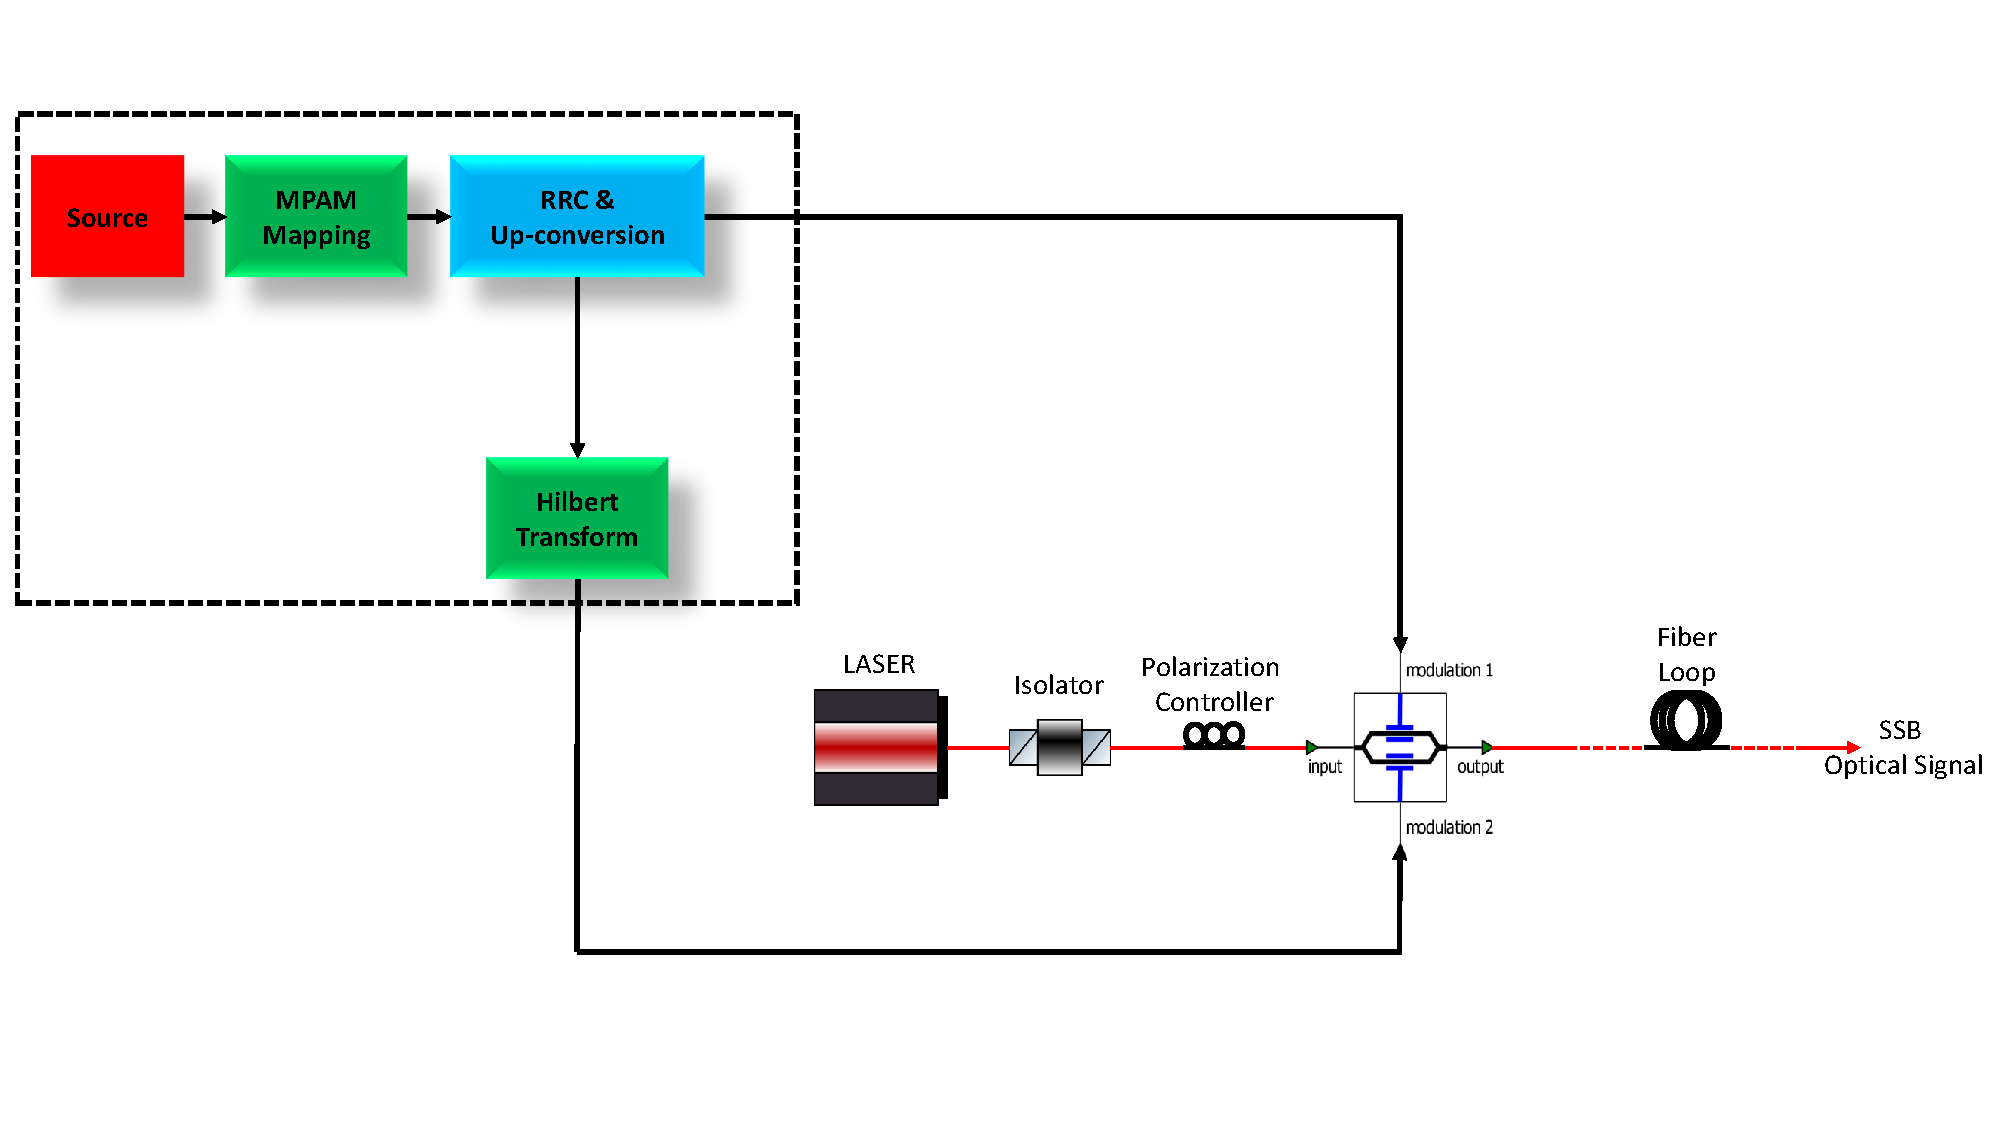
\includegraphics[width=1.0\textwidth, height=7cm]{./sdf/simplified_coherent_receiver/figures/Single_Polarization_Tx.pdf}
	\caption{Transmitter}\label{Transmitter}
\end{figure}

\subsection{KK Scheme}
If we consider the complex envelope of the incoming electric field by $E_s(t)$ confined within the optical bandwidth denoted by B. The LO assumed to be a continuous wave (CW) signal whose amplitude is $E_0$ whose frequency coincides with the left edge of the information-carrying signal spectrum. Here, we assumed that $E_0$ is real-valued and positive, which is equivalent to referring all phase value to that of LO.\\
The complex envelope of the field striking upon the photo-diode can be given as,
\begin{equation}
E(t)=E_s(t)+E_0 exp(i\pi Bt)
\end{equation}
The photo current $I$ produced by the photo-diode is proportional to the field intensity $I=|E(t)|^2$, here proportionality constant considered as 1 for the sake of simplicity. If $E_0$ is large enough to ensure that the signal $E(t)exp(i\pi Bt)=E_0+E_s(t)exp(-i\pi Bt)$ is minimum phase. Equations \ref{Eq:5.15} and \ref{Eq:5.16} can be used to reconstruct the signal $E_s(t)$ as follows:
\begin{equation}
E_s(t)=\{\sqrt{I(t)} exp[i\phi_E(t)]-E_0\} exp(i\pi Bt)
\end{equation}
\begin{equation}
\phi_E(t)=\dfrac{1}{2\pi} p.v. \int_{-\infty}^{\infty} dt' \frac{log[|I(t')|]}{t-t'}
\label{Eq:5.19}
\end{equation}
Here, the average value of the phase returned by Equation \ref{Eq:5.19} is zero, which implies the need for an additional phase-recovery procedure. 
\begin{figure}[h]
	\centering
	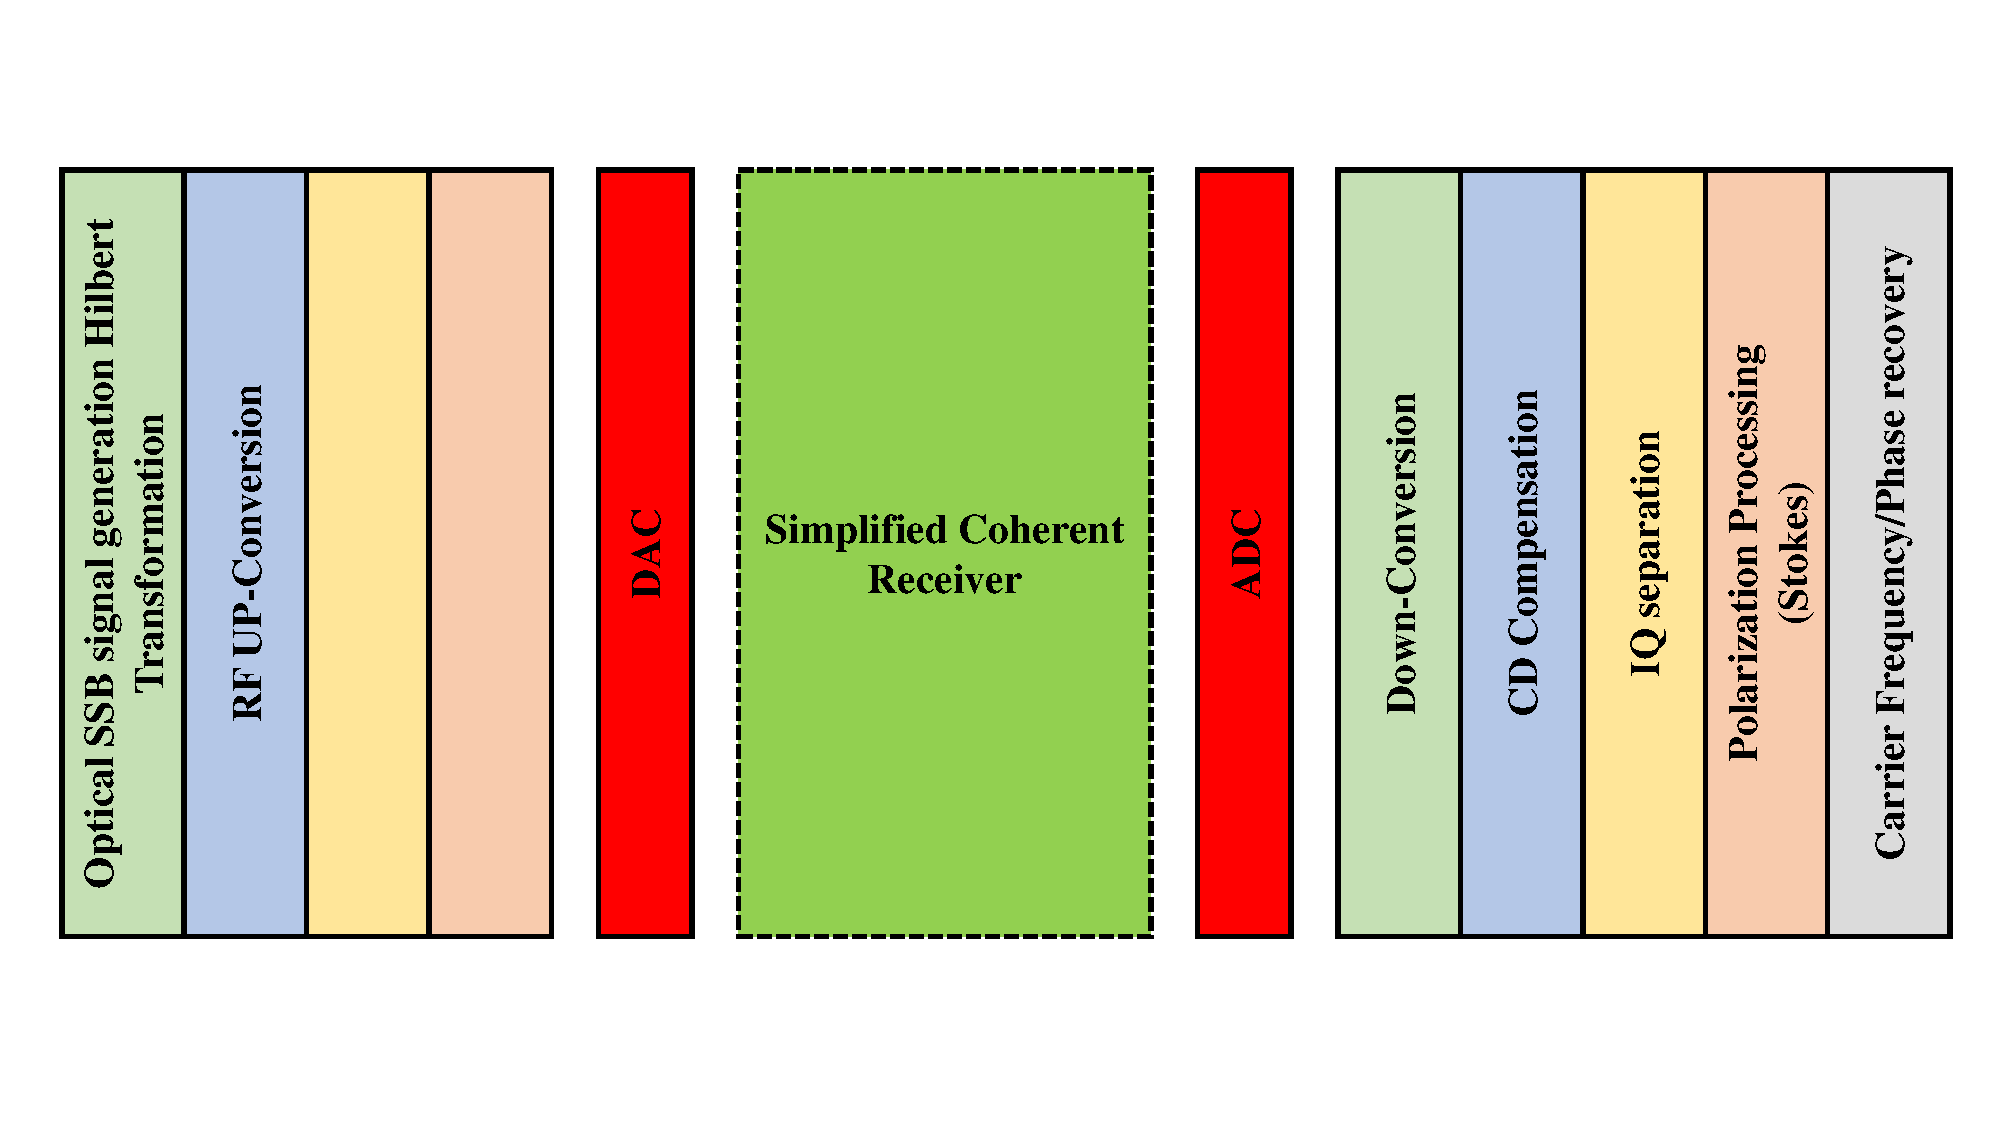
\includegraphics[width=1.0\textwidth, height=8cm]{./sdf/simplified_coherent_receiver/figures/detailed_subsystem.pdf}
	\caption{Tx/Rx DSP main subsystem}\label{DSP_main_subsystem}
\end{figure}

\subsection{Tx side}
Single polarization 16QAM signals (1.25 Gbaud) to be generated at the Tx through an IQ modulator (Figure \ref{DSP_main_subsystem}). The IQ modulated signal is then applied to the Hilbert transformer which generates the imaginary part for our analytical signal. In analytical signal, real and imaginary parts are related to each other by Hilbert transform and it has no negative frequency contents. Such analytical signal can be used for generating bandwidth efficient single sideband (SSB) signal.

\subsection{Rx side}
At the receiver side, signal is coherently detected using a simplified coherent receiver and a local oscillator. The optical signal is then converted into the electrical domain using two balanced photodetector (BPD), or alternatively four photodetector, and amplified by a transimpedance amplifier (TIA). Following that, the signals are sampled by two 8-bit 2.5 GSa/s ADC and the this digitized signal sent to the FPGA (Virtex-7) where all post-detection DSP implemented in real-time.

\begin{thebibliography}{9}
	\bibitem{latexcompanion}
	Antonio Mecozzi, Cristian Antonelli, and Mark Shtaif.
	\textit{Kramers-Kronig Coherent Receiver}.
	Optica, vol.3, no.11, 2016, p.1220., doi:10.1364/optica.3.001220.
	
\end{thebibliography}


